\documentclass[a4paper]{article}

\usepackage{amsmath}
\usepackage{amsthm}
\usepackage{amssymb}

\usepackage{hyperref}
\hypersetup{pdfborder=0 0 0}
\usepackage{url}
\usepackage{floatrow}
\usepackage{esint}
\usepackage{graphicx}
\usepackage{multirow}
\usepackage{multicol}
\usepackage{float}
\usepackage{floatrow}
\usepackage{fancyvrb}

\usepackage{xcolor}

\usepackage{listings}

\setlength{\parindent}{0pt}

\newcounter{list}
\lstnewenvironment{listing}[4][black]
{
	\color{#1!50!black}
	\refstepcounter{list} % this increment the value of counter by one
	\begin{center}
		\textbf{\large{Listing \thelist}}  % this prints the value of the counter
		\textbf{: #2} \\ {\small \textbf{#3}}
	\end{center}
	\lstset{
	language=#4,
	numbers=left,
	breaklines=true,
	keywordstyle=\color{blue}\bfseries,
	numberstyle=\tiny \color{gray},
	commentstyle=\color{green!30!black},
	stringstyle=\color{violet}
	}
}
{
	\vspace{2em}
}

\begin{document}
\title{CS251 Assignment Report}
\author{Aryan Mathe \& Yash Ruhatiya}
\date{22 August}
\maketitle

{\color{blue}\tableofcontents}

\clearpage

\section{Question-1}

\subsubsection{Laplace PDF}
\begin{figure}[H]
	\centering
	\begin{floatrow}
		\ffigbox[10cm]{\caption{Plot}}{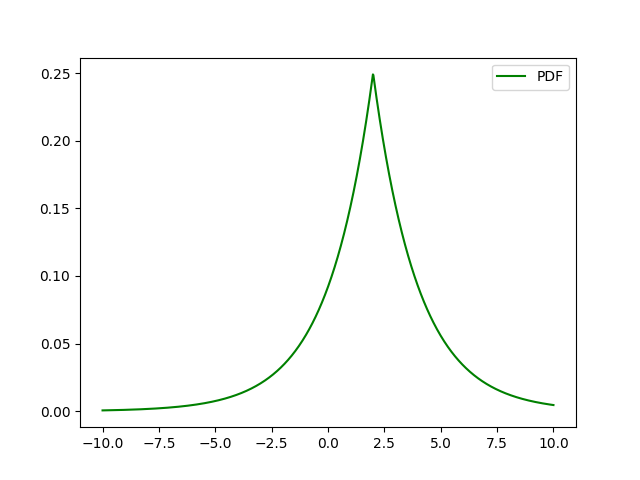
\includegraphics[height=7cm, width=9cm]{lapPDF.png}}
	\end{floatrow}
\end{figure}

\subsubsection{Laplace CDF}
\begin{figure}[H]
	\centering
	\begin{floatrow}
		\ffigbox[10cm]{\caption{Plot}}{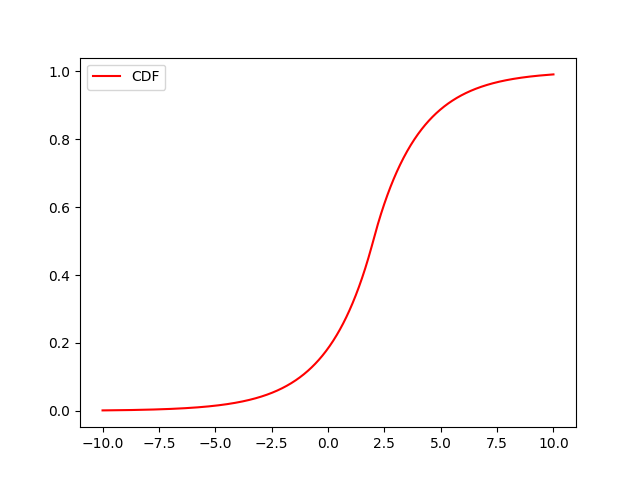
\includegraphics[height=7cm, width=9cm]{lapCDF.png}}
	\end{floatrow}
\end{figure}

\subsubsection{Gumbel PDF}
\begin{figure}[H]
	\centering
	\begin{floatrow}
		\ffigbox[10cm]{\caption{Plot}}{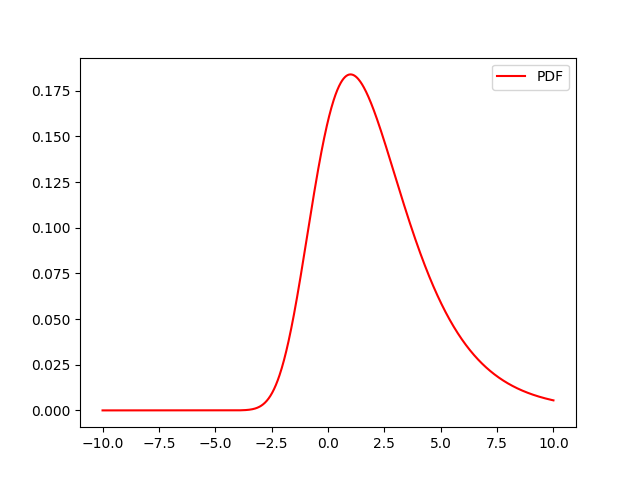
\includegraphics[height=7cm, width=9cm]{gumbPDF.png}}
	\end{floatrow}
\end{figure}

\subsubsection{Gumbel CDF}
\begin{figure}[H]
	\centering
	\begin{floatrow}
		\ffigbox[10cm]{\caption{Plot}}{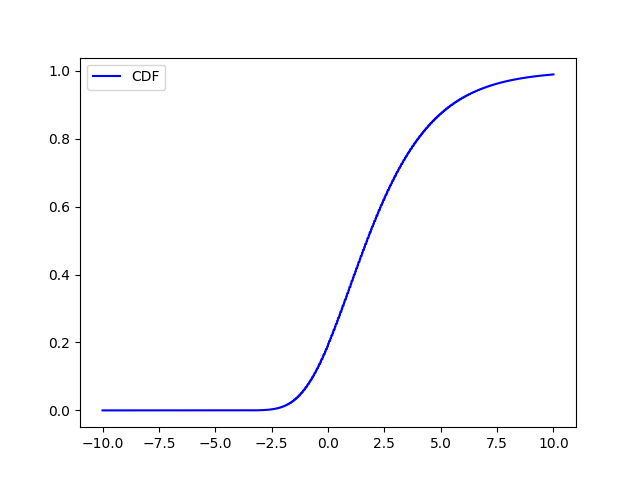
\includegraphics[height=7cm, width=9cm]{gumbCDF.png}}
	\end{floatrow}
\end{figure}

\subsubsection{Cauchy PDF}
\begin{figure}[H]
	\centering
	\begin{floatrow}
		\ffigbox[10cm]{\caption{Plot}}{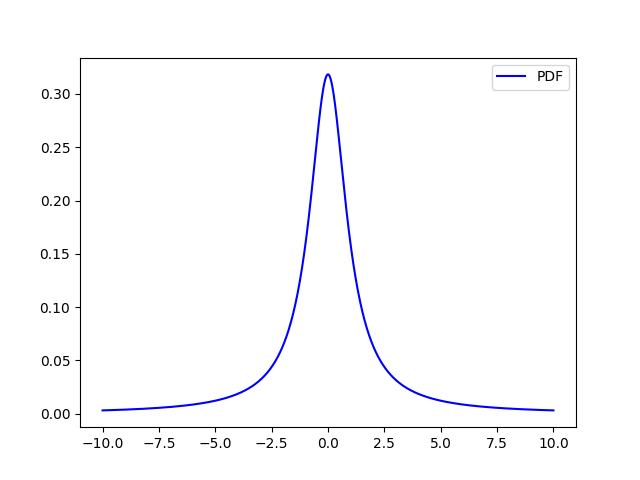
\includegraphics[height=7cm, width=9cm]{cauPDF.png}}
	\end{floatrow}
\end{figure}

\subsubsection{Cauchy CDF}
\begin{figure}[H]
	\centering
	\begin{floatrow}
		\ffigbox[10cm]{\caption{Plot}}{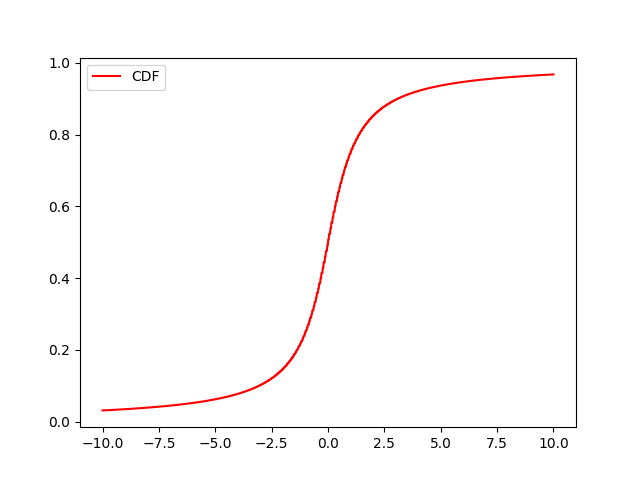
\includegraphics[height=7cm, width=9cm]{cauCDF.png}}
	\end{floatrow}
\end{figure}

\subsubsection{Variances}

\VerbatimInput{varLap.txt}
\VerbatimInput{varGumb.txt}
\VerbatimInput{varCau.txt}
\clearpage


\section{Question-2}


\subsection{Poisson Sum}
\subsubsection{Values for $\hat{P}(Z)$}
Values of $\hat{P}(Z)$ for $k=0, 1 ... ,25$ are:

\VerbatimInput{ques2Sum.txt}

\vspace{1.2em}

\subsubsection{Sum of two Poisson Random Variables}

$P(Z)$ where, $Z=X+Y$ ($X$ and $Y$ are two poisson random variables with average rate $\lambda, \mu$) can be calculated by using the following formula

$$ P(Z=k; \lambda;\mu) = \frac{e^{-(\lambda + \mu)}{(\lambda + \mu)}^{k}} {k!}$$ 
 
\clearpage

\subsubsection{Comparision between Actual and Experimental}
The figure below shows the comparision between $\hat{P}(Z)$ and $P(Z)$ graphically

\begin{figure}[H]
	\centering
	\begin{floatrow}
		\ffigbox[10cm]{\caption{Comparision Plot}}{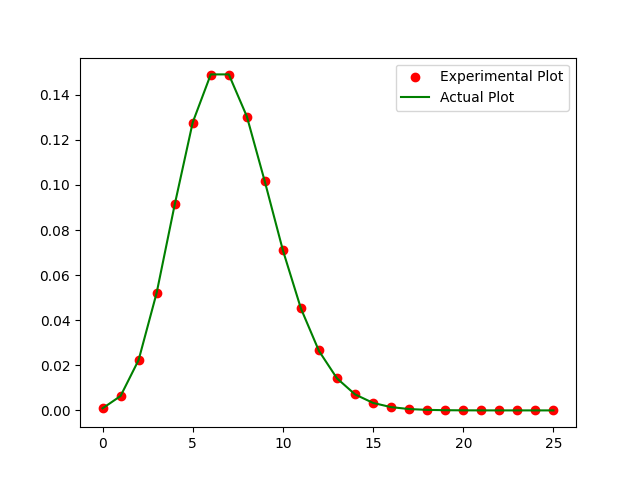
\includegraphics[height=7cm, width=9cm]{ques2Part1.png}}
	\end{floatrow}
\end{figure}

\subsection{Poisson Thinning}

\subsubsection{Values for $\hat{P}(Z)$}

Values of $\hat{P}(Z)$ for $k=0, 1 ... ,25$ are:

\VerbatimInput{ques2Thin.txt}

\subsubsection{Thinned Poisson Variable}

$P(Z)$ where, $Z$ is the thinned random variable out of Y ($Y$ is a poisson random variable with average rate $\lambda$ and $p$ is the probability parameter) can be calculated by using the following formula

$$ P(Z=k; \lambda; p) = \frac{e^{-\lambda p}{(\lambda p)}^{k}} {k!}$$

\subsubsection{Comparision between Actual and Experimental}
The figure below shows the comparision between $\hat{P}(Z)$ and $P(Z)$ graphically

\begin{figure}[H]
	\centering
	\begin{floatrow}
		\ffigbox[10cm]{\caption{Comparision Plot}}{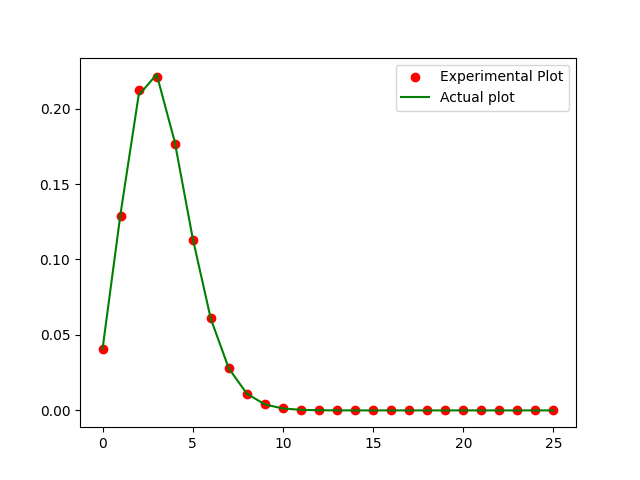
\includegraphics[height=7cm, width=9cm]{ques2Part2.png}}
	\end{floatrow}
\end{figure}


\clearpage

\section{Question-3}
\subsubsection{Random Walk Position Plot}
\begin{figure}[H]
	\centering
	\begin{floatrow}
		\ffigbox[8cm]{\caption{Position Histogram}}{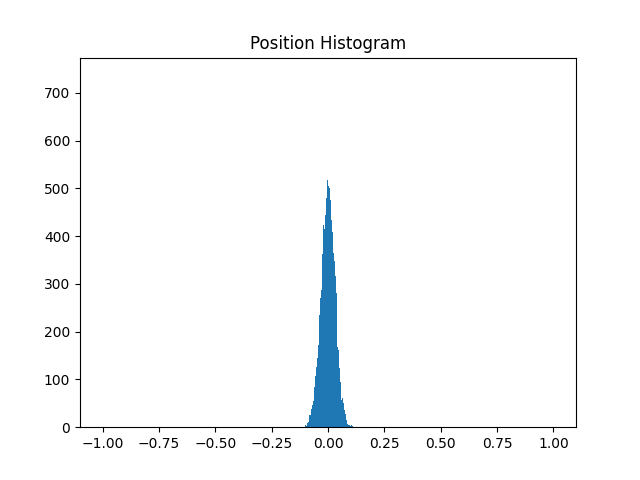
\includegraphics[height=8cm, width=8cm]{ques3Part1.png}}
	\end{floatrow}
\end{figure}

\subsubsection{Random Walk Space -Time Plot}
\begin{figure}[H]
	\centering
	\begin{floatrow}
		\ffigbox[8cm]{\caption{Space Time Plot}}{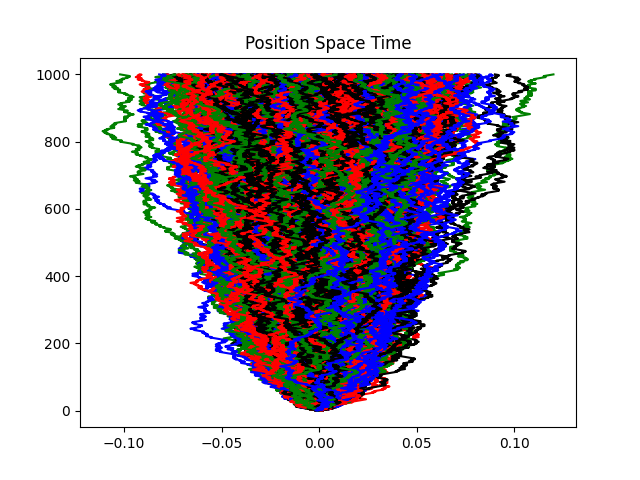
\includegraphics[height=8cm, width=8cm]{ques3Part2.png}}
	\end{floatrow}
\end{figure}

\subsubsection{Law of Large Numbers}
\vspace{1em}
{\textbf{Mean}}\\
Acccording to the \textbf{Law of Large Numbers}, the average of the results obtained from a large number of trials tends to the expected value as more trials are performed.

$$\lim_{n \to \infty} \sum_{i=1}^{n} \frac{X_i}{n} = \overline{X} = E(X)$$

{\textbf{Variance}}\\
Expected Variance $\hat{V}(X)$ tends to true variance $V(X)$ when the number of elements $N$ tends to $\infty$ \\\

Here $\hat{M}$ is the expectation value for the random variables $M:= E[X]$\\

$$\hat{V}(X) = \frac{\sum_{i=1}^{N}(X_{i} - \hat{M})^2}{N}$$
$$\hat{V}(X) = \frac{\sum_{i=1}^{N}(X_{i}^2 + \hat{M}^2 - 2\hat{M}X_{i})}{N}$$
$$\hat{V}(X) = \frac{\sum_{i=1}^{N}X_{i}^2}{N} + \hat{M}^2 - 2\hat{M}^2$$
$$\hat{V}(X) = \frac{\sum_{i=1}^{N}X_{i}^2}{N}  - \hat{M}^2$$

Now using the \textbf{Law of large numbers} on random variable $X_{i}^2$, the expression 
$\frac{\sum_{i=1}^{N}X_{i}^2}{N}$ reduces to $E[X^2]$

$$\hat{V}(X) = E[X^2]  - \hat{M}^2$$


So the expected variance $\hat{V}(X) = Var(X)$ as $N$ tends to $\infty$.

\subsubsection{Empirically Computed Mean and Variance}
\vspace{1em}
\VerbatimInput{ques3MeanVar.txt}

\subsubsection{True Mean and Variance}

Let the random variable for position be $X$, $\Delta z$ be the step width, $p$ be the probability of moving left, $n$ be the total number of steps, and  $x$ be the number of left steps taken by the walker.\\

{\textbf{Mean}}\\
Then the final position $z$ is given as $z=\Delta z(2x-n)$

$$E(Z = \Delta z(2x-n)) = 2\Delta z E(x) - n\Delta z$$
We know that the expected value for the binomial distribution is given as $E(X) = np$, which implies
$$ E(Z) = n\Delta z(2p-1)$$

Since for a uniform distribution $p=0.5$
$$E(Z) = 0$$

{\textbf{Variance}}\\
$V(Z)$ denotes the variance for the distribution of Z,\\
$$V(Z=\Delta z(2x-n)) = \frac{\sum_{z} \left(z - E(Z)\right)^{2}}{n}$$
$$V(Z=\Delta z(2x-n)) = \frac{\sum_{x} \left(\Delta z(2x-n) - n\Delta z(2p-1) \right)^{2}}{n}$$

$$V(Z=\Delta z(2x-n)) = \frac{\sum_{x} \left(2\Delta z(x-np)\right)^{2}}{n}$$

$$V(Z=\Delta z(2x-n)) = 4\Delta z^{2} \frac{\sum_{x} \left(x-np\right)^{2}}{n}$$\\


Now we know, $V(X) = np(1-p)$ for a binomial distribution.
$$V(Z)=4\Delta z^{2}(np(1-p))$$

\subsubsection{Error in Mean and Variance}
\vspace{1em}
\VerbatimInput{meanVarError.txt}

\clearpage

\section{Question-4}
\subsection{Plots}

\subsubsection{Histogram for M-Shaped Distribution}
\begin{figure}[H]
	\centering
	\begin{floatrow}
		\ffigbox[7cm]{\caption{Histogram}}{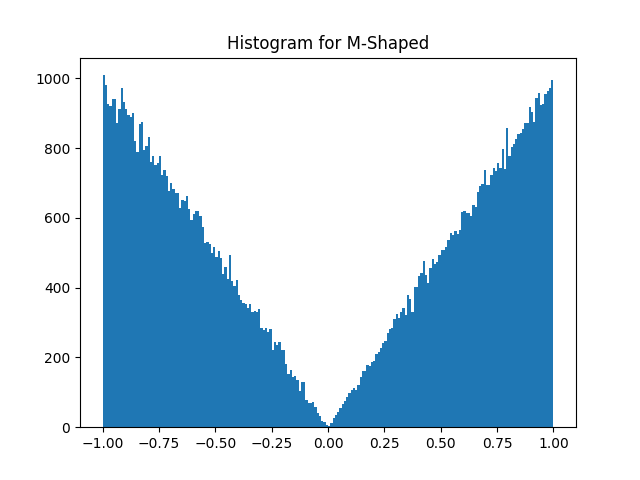
\includegraphics[height=6cm, width=7cm]{ques4Hist.png}}
	\end{floatrow}
\end{figure}

\subsubsection{CDF for M-Shaped Distribution}
\begin{figure}[H]
	\centering
	\begin{floatrow}
		\ffigbox[7cm]{\caption{CDF Plot}}{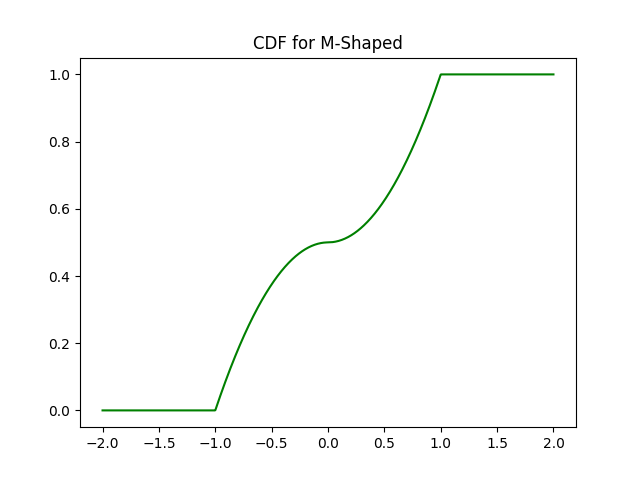
\includegraphics[height=6cm, width=7cm]{ques4CDF_M.png}}
	\end{floatrow}
\end{figure}

\subsubsection{Histograms for Average M-Shaped Distribution}
\begin{figure}[H]
	\centering
	\begin{floatrow}
		\ffigbox[14cm]{\caption{Histograms}}{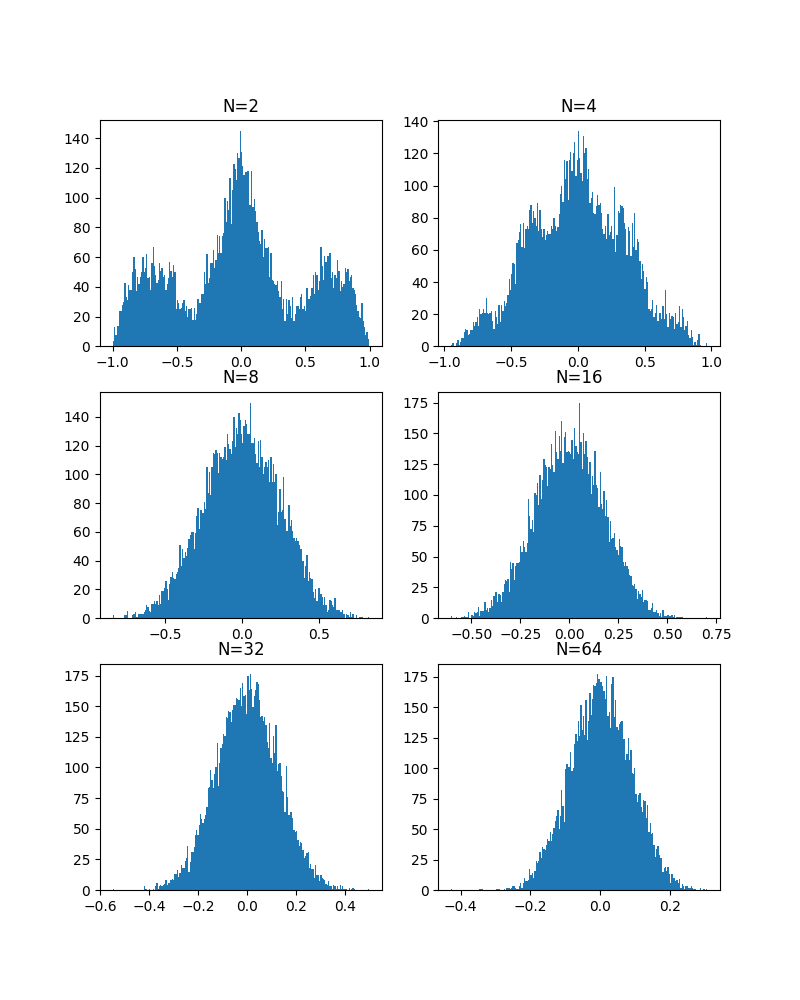
\includegraphics[height=14cm, width=14cm]{avg_M_for_N.png}}
	\end{floatrow}
\end{figure}

\subsubsection{CDFs for Average M-Shaped Distribution}
\begin{figure}[H]
	\centering
	\begin{floatrow}
		\ffigbox[7cm]{\caption{CDF Plots}}{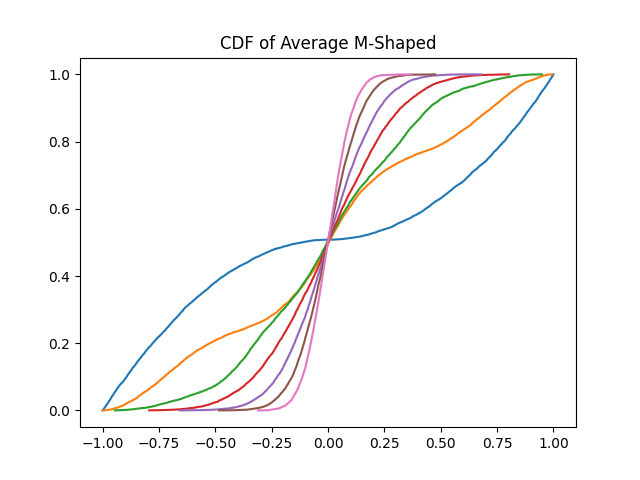
\includegraphics[height=7cm, width=7cm]{CDF_avg_M.png}}
	\end{floatrow}
\end{figure}


\section{Question-5}
\subsubsection{Unifrorm Distribution Error - Box Plot}
\begin{figure}[H]
	\centering
	\begin{floatrow}
		\ffigbox[14cm]{\caption{Error Boxplot}}{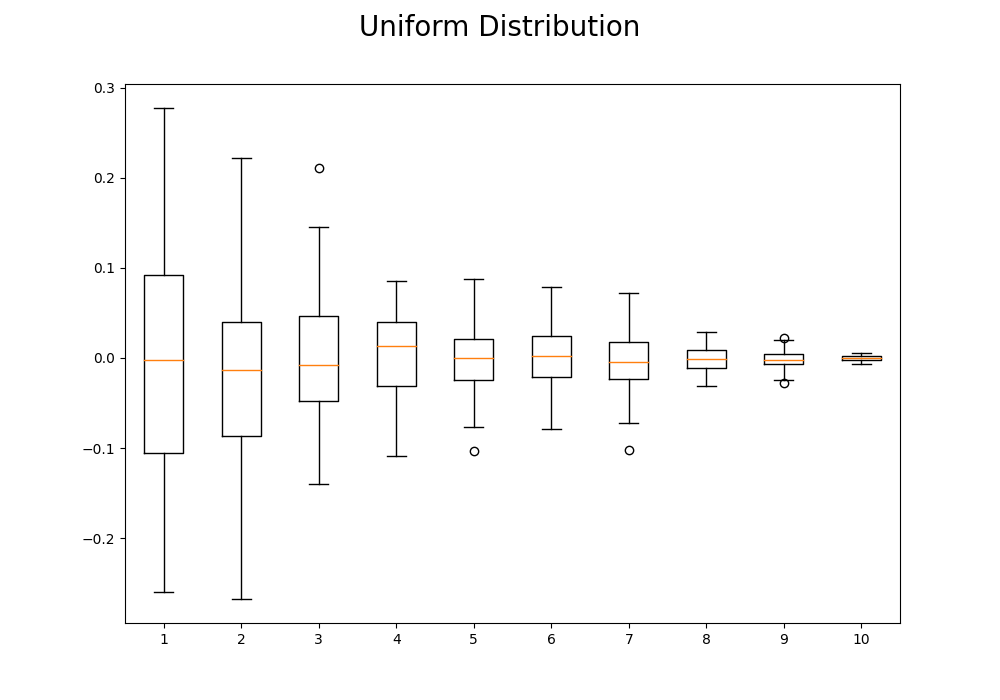
\includegraphics[height=12cm, width=14cm]{boxUni.png}}
	\end{floatrow}
\end{figure}


\subsubsection{Gaussian Distribution Error - Box Plot}
\begin{figure}[H]
	\centering
	\begin{floatrow}
		\ffigbox[14cm]{\caption{Error Boxplot}}{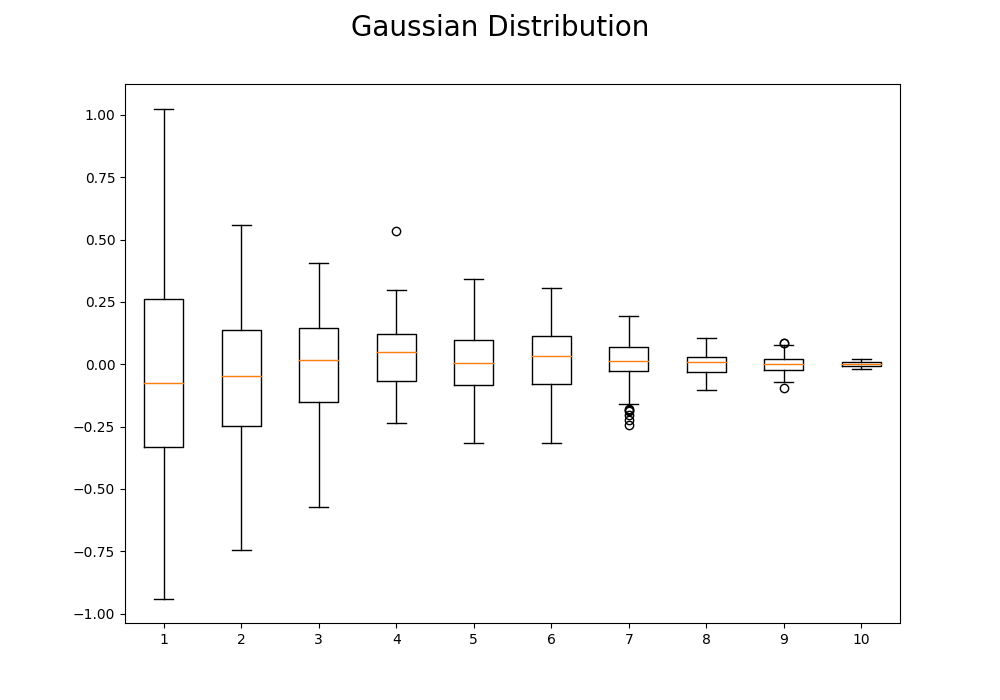
\includegraphics[height=12cm, width=14cm]{boxGaus.png}}
	\end{floatrow}
\end{figure}

\subsubsection{Interpretaion from Plot}
Here boxplots represents the error distibution. \\ \\
It can be clearly observed from the boxplots that the variance of the error distribution keeps on decreasing and keeps on converging to a smaller value.\\
So as $N$ increases and tends to $\infty$ the error and its variance converges to $0$ for both \textbf{uniform} and \textbf{gaussian} distributions.


\clearpage

\centering
{\Huge \textbf{End of Report}}

\end{document}